% toggles back at the end of this file!
\changemenucolor{gray}{bg}{named}{ese_bg_color} %background of the menukeys
\changemenucolor{gray}{br}{named}{ese_fg_color} %border of the menukeys
\changemenucolor{gray}{txt}{named}{ese_fg_color} %text of the menukeys

\newcommand{\semester}[1]{\minisec{\Large\vspace{.7\baselineskip} #1 Semester\\[.6\baselineskip]}}
\newcommand{\modul}[1]{\vspace{.5\baselineskip}\textbf{\menu[;]{#1\,}}\\[.2\baselineskip]}

\chapter{Module overview}

Here you will find a short overview of the modules you will attend during your studies. The order is not binding, it is only the recommended path through the program.
The symbols \textbf{\menu[;]{I;M;D}} indicate the modules for Bachelor of Computer Science, Bachelor of Media Informatics and Diploma of Computer Science respectively.

\vspace*{-1em}

\semester{1st}

\modul{I; M; D; Einführung in die Mathematik für Informatiker}
You know your way around matrices?
Then you know what to do with the terms determinant, diagonalizability, scalar product and the solution of a homogeneous linear system of equations -- if not, then you will learn it here from scratch.
In addition, in discrete mathematics, the times and pluses are virtually redefined and you learn to think a little differently.

\modul{I; M; D; Algorithmen und Datenstrukturen}
\label{sec:aud}
What comes first?
5 or 3?
Such questions will keep you busy in Algorithmen und Datenstrukturen as you learn about quicksort, heapsort and the like.
% Der Wortwitz gefällt mir...
You will also try your hand at gardening, growing AVL and other trees.
In the process, you will get acquainted with the C programming language.

\modul{I; M; D; Einführungspraktikum}
Have you always loved playing with Lego?
Then you will like this internship, which takes place during the lecture-free period.
As part of a team, you will be given the task of teaching a self-designed robot in Python how to find its way around a maze on its own.
In the process, and in the competition that follows, there is no shortage of fun.
For diploma students, there is an additional one-week individual project, the so called Strategiespiel internship, where you can show what you've got in C or optionally C++. If necessary this internship can be postponed to the summer semester.
In recent years, participants had to write an artificial intelligence for a predetermined well-known board game

\newpage

\modul{I; M; Einführung in die Medieninformatik}
\label{lec:emi}
In this module you will learn how human perception works and how you can design software ergonomically.
In addition, you will be introduced to various properties of information and data formats based on the media comprising text, images, audio and video.
In the section about texts and images, the corresponding document formats of the Internet (HTML and SVG) will be discussed.
You can also expect a short excursion into app development.
Another part of the module gives an overview of document processing using XML techniques.
In tutorials and in the form of a project in a small group over the course of the semester, you will have the opportunity to put what you have learned directly into practice.

\modul{D; Technische Grundlagen und Hardwarepraktikum}
If you've always wanted to know what the electrons in your home computer have to go through, you'll learn exactly that here.
Initially you will look at transistor, diode and operational amplifier circuits.
Based on this, you will take a closer look at logic elements and complex circuits.
In the following semester, you will be able to apply all that you have learned here to plug together a few circuits yourself.

\modul{D; Rechnerarchitektur}
This is about the basic building blocks of a computer:
Memory, bus systems, arithmetic and control units.
Read binary code? All nonsense! In this module you will learn what machine language really looks like and get a crash course in assembler.
You'll also look at the pipelining principle and be confronted with the problems that arise with it.
Finally, we will discuss which methods you can use to accelerate today's computer architectures and to use parallel architectures.

\vfill

\begin{figure}[h!]
\centering
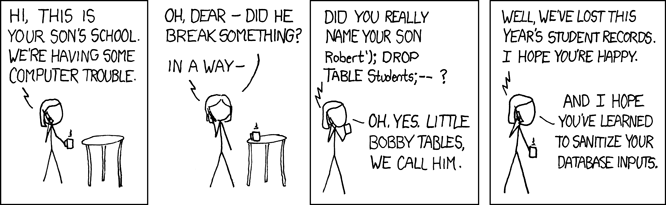
\includegraphics[scale=.5]{img/xkcd/exploits_of_a_mom.png}
\caption*{{\small \textit{Her daughter is named Help I'm trapped in a driver's license factory. (https://xkcd.com/327)}}}
\end{figure}

\semester{2nd}

\modul{I; M; D; Mathematische Methoden für Informatiker}
After the a-level material has sunk in much deeper than before, the next two semesters will take you into new areas of mathematics.
Initially, you'll study the different types of algebraic structures (which are sets of arbitrary symbols and arithmetic operations declared on them).
Vectors, matrices, and fields follow.
Then comes a jump from the discrete to the continuous.
Calculus is not as boring as in school, there is also a version with multiple variables.
The whole thing culminates in the introduction of differential equations.
Towards the end you turn again to polynomials.
First, efficient approximation methods are dealt with, later a short excursion into stochastics ensues.

\modul{I; M; D; Programmierung}
You probably already knew that programming languages don't grow on trees, but here you will learn that they follow strict mathematical rules.
Using a part of the programming language C as an example, the syntax is first defined with the help of grammars.
Shortly after, you will come into contact with the functional programming language Haskell and get to know a completely new approach to programming.
Through many nice, recursively nested mappings, the semantics is then defined, i.e.\ the effect that such a program has on an (abstract) computing machine.
In addition, you will learn how to formally prove the correctness of a program fragment.

\modul{I; M; D; Softwaretechnologie}
Developing software is an art and writing good software is not an easy thing -- if you haven't already -- you will realize this once you reached this module.
To be able to demonstrate this skill, you need some tools of the trade, which you will get here.
You will be introduced to helpful concepts through Java and design procedures alongside professional documentation.
This will lay the foundation for the project in the third semester, where you can earn laurels in project management and software development.


\newpage

\modul{I; D; Informations- und Kodierungstheorie}
What information actually is and what constitutes it will occupy you here.
At the beginning, the focus is on how you can represent and store information.
A little later, it will be explained to you why and how the information is protected by means of coding, so that it arrives at you safely when it is exposed to interference and manipulation on the way.
The knowledge you have acquired in mathematics so far will be of use to you.

\modul{I; Einführung in die Computergraphik}
\label{lec:ecg}
What is actually behind the Unreal Engine? How do shaders work?
Why do the characters in computer games look more and more realistic?
You'll find out in this module, along with the structure of graphics systems, color spaces, raster graphics and their applications.
Existing problems such as aliasing and artifacts are included, as well as their algorithmic solutions.
C++ is used as the programming language for the exercises.

\modul{M; Grundlagen der Gestaltung}
In this module you will learn terminology and general principles of design.
The course is deliberately limited to two-dimensional areas.
Form categories, contrast formation and color theory form the main focus.
The accompanying exercises are designed to give you an insight into the subject matter and to awaken your sensitivity through manual work.

\modul{M; Medien und Medienströme}
Here you will learn about media, their compression and editing.
The application of various tools for the creation of media and their characteristics are also the subject of this course.
Thus, you will deal with the basics of image, audio and video processing in the form of exercises.

\modul{D; Rechnerarchitektur}
Continuation of the 1st semester.

\modul{D; Technische Grundlagen und Hardwarepraktikum}
Continuation of the 1st semester. Circuit diagrams and physical laws -- all well and good. But how does it all fit together?
That's what this module is all about. In a series of experiments, you'll put everything you've learned into practice.
From analog to digital to your own little computer, everything is included!

\newpage

\semester{3rd}

\modul{I; M; D; Mathematische Methoden für Informatiker}
Continuation of the 2nd semester.

\modul{I; M; D; Softwaretechnologie-Projekt}
The project takes up most of the third semester.
Here you have to put your knowledge from the course \enquote{Softwaretechnologie} into practice.
In a team of five you have the task to write an application for a real clientele or the chair.
As a team, you will have to take care of the conception, planning, programming and division of labor.
You consult with the clientele and/or the supervisors and maybe you have to change everything again.
The module ends with the presentation of the finished product.
At the end you will have an impression of what working in IT can look like.

\modul{I; M; D; Formale Systeme}
True?
And or false?
What is false becomes, if it is false false, true?
Logical!
If everyone has an umbrella tomorrow, will it rain?
Besides propositional logic, this module teaches you the basics of formal languages.
This is followed by thoughts on machine computability and automata theory.
Turing sends his regards.

\modul{I; M; Rechnerarchitektur}
See 1st semester for description.

\modul{I; Technische Grundlagen und Hardwarepraktikum}
See 1st semester for description.

\modul{M; Einführung in die Mediengestaltung}
The lecture will teach you the basics of multimedia design from the point of view of the development of individual directions (film, Internet) with reference to the design changes in the past centuries (book).
In addition, you will learn the useful method of metaphor formation and key aspects of interface design.

\newpage

\modul{D; Grundlagen des Nebenfachs}
Depending on which minor you choose, you will deal with topics that are only remotely related to computer science.
Think outside the box and get to know other worlds is the motto.
Here you have the opportunity to get to know students from other disciplines.

\modul{D; Betriebssysteme und Sicherheit}
In this course, you'll take a close look at the servant spirits that toil between the hardware and the colorful applications.
Why can you use a computer to write text, compile code, edit an image, and listen to music all at the same time?
How is your data protected in computer systems?
Why are so many people into this Unix here?

\semester{4th}

\modul{I; M; D; Datenbanken und Rechnernetze}
Where do you put your 20 terabytes of user data? And how does the YouTube video actually get from the USA to your browser?
This is the topic of this module, which consists of two different courses.
In \textit{Datenbanken} you will first learn methods for efficient data storage.
After that, you will be taught how to design and create complex relational databases yourself.
In \textit{Rechnernetze} you will start with the working principles of modems and network cards and you will get a short overview of modern communication and switching protocols.
Also the sector of mobile communication and the difficulties that arise in it are briefly examined.

\modul{I; M; Rechnerarchitektur}
Continuation of the 3rd semester.

\modul{I; D; Theoretische Informatik und Logik}
The continuation of Formale Systeme.
Thus, you consider the correctness and scheduling of algorithms and their necessary effort in terms of time and space requirements.
A detour into predicate logic and logic programming rounds off the module.

\modul{I; Technische Grundlagen und Hardwarepraktikum}
Continuation of the 3rd semester.

\modul{M; Medienpsychologie und -didaktik}
Mediendidaktik is the \enquote{art of teaching}.
Here you will find answers to the questions:
What is education?
How does it proceed?
How can it be improved?
You will learn about the development of teaching methods.
In the parallel internship, you will apply what you have learned to the development of an educational game.

\modul{M; Informations- und Kodierungstheorie}
See 2nd semester for description.

\modul{M; Einführung in die Computergraphik}
See 2nd semester for description.

\modul{M; Medieninformatik-Projekt}
The big highlight of Medieninformatik in the bachelor's degree.
In small groups you have to realize a mobile game, an internet page or something else multimedia.
Apart from the task, there are virtually no limits to your imagination.
It's all about hard work, team spirit and dealing with sleep deprivation when the deadline finally approaches.

\modul{D; Grundlagen des Nebenfachs}
Continuation of the 3rd semester.

\modul{D; Allg. Basisqualifikationen}
English is the only relevant language for computer science.
Here you will learn how to express yourself professionally in English.
If you are already satisfied with your English skills, you can alternatively attend another language course or any course from the university-wide Studium Generale program.
In addition to the two compulsory language courses, there is also a proseminar.
There you will learn \textit{how} to prepare a scientific publication -- by writing and presenting one yourself on a topic of your choice.

\modul{D; Forschungslinie}
Here you will get an overview of current research topics and learn how to work in a research-oriented way.
This module will help you to choose the right specialization later on. Attending this course is also interesting for bachelor's and master's students, as they also have to deepen their knowledge eventually.

\begin{figure}[b!]
\centering
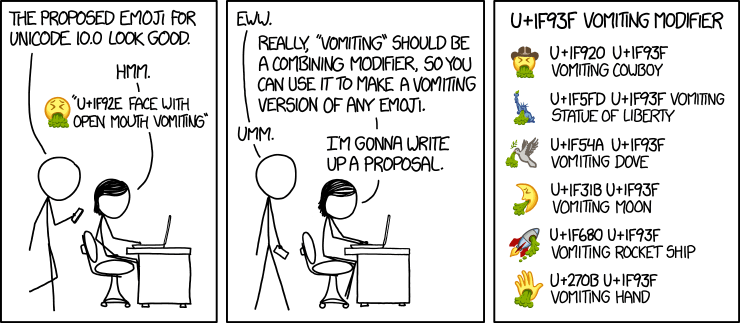
\includegraphics[scale=.4]{img/xkcd/vomiting_emoji.png}
\caption*{{\small \textit{My favorite might be U+1F609 U+1F93F WINKING FACE VOMITING\@. (https://xkcd.com/1813)}}}
\end{figure}
\pagebreak
\semester{5th}

\modul{I; M; Vertiefung in der Informatik/Medieninformatik}
Here you can choose suitable events from a catalog of courses to broaden your scientific horizons.
The options include lectures, tutorials, internships, excursions, seminars and more.

\modul{I; M; Betriebssysteme und Sicherheit}
See 3rd semester for description.

\modul{I; D; Intelligente Systeme}
This module is about artificial intelligence.
Here you will learn problem solving, knowledge representation, planning, and language processing.
Why could IBM's Watson win in \textit{Jeopardy!} against the best human gamers?
How does a spam filter know what is spam and what is not?
You'll learn the answers with the learning algorithms used to find them.

\modul{I; D; Systemorientierte Informatik/Hardware Software Codesign}
This module deals with interfaces between computers and industrial systems.
First, you will abstract what is common to all systems encountered, and terms such as \enquote{system}, \enquote{signal}, and \enquote{control loop} will be formalized to make it easier to work computationally.
You will be made fit for analyzing and predicting transmission behavior and responses that such a system will exhibit given a particular input.
Aspects of audio and video technology such as digitization and filtering are also covered.

\modul{M; Web- und Multimedia Engineering}
How can you make the web multimedia and interactive with today's technology? Why is HTML5 so great?
How do you use professional development tools and appropriate languages to project your imagination into the result?
This module helps to learn appropriate methods and gain experience in using them.

\modul{M; Medieninformatik-Projekt}
Continuation of the 4th semester.

\modul{D; Vertiefung im Nebenfach}
Now that you've learned the basics of your chosen minor, it's time to get serious and dig deeper.

\modul{D; Basismodul 1, 2 und 3}
Here you choose three of seven different topics and deal with them.
You can choose between Applied Computer Science, Artificial Intelligence, Software and Web Engineering, System Architecture, Computer Engineering, Theoretical Computer Science and Computer Graphics.
Within these directions, you can choose suitable courses.

\semester{6th}

\modul{I; M; Spezialisierung in der Informatik/Medieninformatik}
Further in-depth study following the same pattern as in the fifth semester in preparation for the bachelor thesis.

\modul{I; M; Überfachliche Qualifikation}
\label{lec:aqua}
In this type of minor, you'll orient yourself to topics of your interest across disciplines to develop subject-specific expertise.
Plus, this module is another good time to learn a new language. Japanese? Arabic? Russian? Or English again?
Again, courses can be chosen from a catalog.

\newpage

\modul{I; M; Bachelorarbeit und Kolloquium}
As a crowning finale, you will complete your Bachelor's thesis on a topic of your choice and defend it in a presentation.
Congratulations! You are now officially \textit{Bachelor of Science}! How about a Master's degree afterwards?

\modul{D; Vertiefung im Nebenfach}
Continuation of the 5th semester.

\modul{D; Basismodul 1, 2 und 3}
Continuation of the 5th semester.

\semester{7th\ to 10th}

In the computer science diploma program, you have four more semesters to go after the first six. At the same time, most bachelor's students will choose a master's program.
During the seventh semester, you will complete a professional internship, which is also an ideal opportunity for a stay abroad.
In the eighth and ninth, you will then select modules that interest you, descend deeper into the abysses of your chosen topic, acquire further skills according to the same principle as in \enquote{Allgemeine Basisqualifikationen}, write a \enquote{Großen Beleg} (comparable to the bachelor's thesis) and complete further work.
And in the tenth, last semester you finally write your diploma thesis and that's it!
That's how fast it can go.

\begin{figure}[b!]
\centering
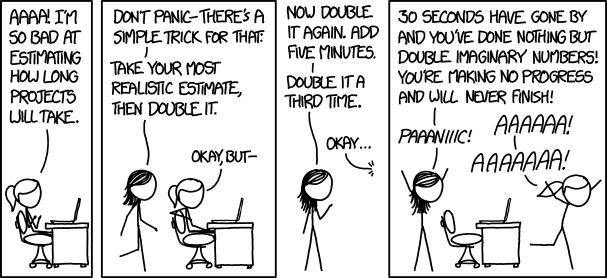
\includegraphics[width=.73\textwidth]{img/xkcd/estimating_time.png}
\caption*{\centering {\small \textit{Corollary to Hofstadter's Law: Every minute you spend thinking about Hofstadter's Law is a minute you're NOT WORKING AND WILL NEVER FINISH\@! PAAAAAANIIIIIIC\@! (https://xkcd.com/1658/)}}}
\end{figure}

\changemenucolor{gray}{bg}{named}{ese_fg_color} %background of the menukeys
\changemenucolor{gray}{br}{named}{ese_bg_color} %border of the menukeys
\changemenucolor{gray}{txt}{named}{ese_bg_color} %text of the menukeys
